\section{Evaluation}
\label{sec:eval-cloak}

In this section, we evaluate \system's efficacy in protecting artists from
style mimicry. We first describe the datasets, models, and experimental
configurations used in our tests. Then we present the results of \system's
protection in a variety of settings. Due to \system's highly visual nature,
we evaluate its performance using both direct visual assessment by
\textbf{human artists} in a user study, and \textbf{automated metrics} (see
\S\ref{sec:metrics} for details).

\para{Summary of results.} Over $93\%$ of artists surveyed believe \system{}
effectively protects artists' styles from AI style mimicry
attacks. Protection efficacy remains high in challenging settings, like when
the mimic has access to unprotected artwork. \system{} also achieves high
protection performance against a real-world mimicry-as-a-service platform. Of
our $1156$ artist participants, over $92\%$ found the perturbations
introduced by cloaking small enough not to disrupt the value of their art,
and over $88\%$ would like to use \system{} to protect their own artwork from
mimicry attacks.

\secspace
\subsection{Experiment Setup}
\label{sec:cloak-setup}

\para{Mimicry dataset. } We evaluate \system's performance in protecting the styles of the following two groups of artists: 

\vspace{-0.2cm}
\begin{packed_itemize}
\item {\em Current artists}: $4$ professional artists let us use their
  artwork in our experiments. These artists have different styles and
  backgrounds (\eg full-time/freelancers, watercolor painters/digital
  artists, well-known/independent). Each provided us with between $26$ to
  $34$ \textit{private} original art pieces for our experiments. We use
  perceptual hashing~\cite{ke2004efficient} to verify that none of these are
  included in existing public datasets used to train generic text-to-image
  models (e.g.~\cite{schuhmann2022laion,changpinyo2021conceptual}).  

\item {\em Historical artists}: We also evaluate \system{}'s protection on
  $195$ historical artists (\eg van Gogh, Monet) from the WikiArt
  dataset~\cite{saleh2015large}. The WikiArt dataset contains 42,129 art
  pieces from $195$ artists. Each art piece is labeled with its genre (\eg
  impressionism, cubism). We randomly sampled $30$ art pieces from each
  artist to use in style mimicry attacks. Generic text-to-image models found
  online have been trained on some artwork from these artists. Using this art
  simulates a more challenging scenario in which a famous artist attempts
  to disrupt a model that already understands their style.
\end{packed_itemize}
\vspace{-0.2cm}

\para{Mimicry attack setup. } We recreate the strongest-possible mimicry
attack scenario, based on techniques used in real-world mimicry
incidents~\cite{ruiz2022dreambooth,sam-steal,hollie-steal},
that works as follows. First, we take art pieces from the victim artist $V$
and generate a text caption for each piece using an image captioning
model~\cite{luo2022vc}. \revise{The pretrained image captioning model generates a short 
sentence to describe the image. We found that this model can correctly caption protected images (examples in Figure~\ref{fig:data-examples}), likely because \system{} focuses on perturbing style features while the captioning models focus on image content.} Then, we append the artist's name to each caption,
\eg ``mountain range \textit{by Vincent van Gogh}''. Finally, we fine-tune a pre-trained generic text-to-image model
(details below) on the caption/image pairs. 

We use $80\%$ of the art pieces from the victim artists to fine-tune models
that mimic each artist's style, reserving the rest for testing. We fine-tune
for $3000$ optimization steps, which we find achieves the best mimicry
performance (Figure~\ref{fig:success-iter} in Appendix). We then use the
fine-tuned, style-specific model to generate mimicked artwork in style of
each victim artist. We query the model using the generated captions (which
include $V$'s name) from the held-out test artwork set. We generate $5$
pieces of mimicked art for each text caption using different random seeds and
compare these to the real victim art pieces with this caption. Additional
details on training and generation parameters, as well as its sensitivity to
random seed selection and the number of training art pieces are in Appendix~\ref{app:mimicry}.  

% Fine-tuning a style-specific mimicry model takes 56.4 minutes on average on one Titan RTX GPU~\footnote{This takes longer than real-world mimicry incidents because we finetune more steps for better mimicry performance.}. 

\para{Text-to-image models.} We use two state-of-the-art, public, generic text-to-image models in our experiments: 

\vspace{-0.2cm}
\begin{packed_itemize}
\item \textit{Stable Diffusion (SD)}: Stable Diffusion is a popular and
  high-performing open-source text-to-image model~\cite{stable2-1},trained
  on 11.5 million images from the LAION dataset~\cite{schuhmann2022laion}. SD
  training takes over 277 GPU months (on A100 GPU) and costs around
  \$600K~\cite{stable2-1}. SD uses diffusion methods to generate images and
  achieves state-of-the-art performance on several
  benchmarks~\cite{rombach2022high}. Viewed as one of the best open-source
  models, SD has powered many recent developments in text-to-image
  generation~\cite{blender-plugin,novelai-update,gimp,aigame}. We
  use SD version 2.1 in the paper~\cite{stable2-1}, the most up-to-date
  version as of December 2022.  

\item \textit{DALL$\cdot$E-mega (\dalleM)}: \dalleM-mega, an updated version
  of the more well-known \dalleM-mini, is an open-source model based on
  OpenAI's \dalleM~1~\cite{ramesh2021zero}. The model leverages a VAE for
  image generation and is trained on 17 million images from three different
  datasets~\cite{sharma-etal-2018-conceptual,changpinyo2021conceptual,thomee2016yfcc100m}. Training
  takes 2 months on 256 TPUs~\cite{mini-training}. While \dalleM~ performs
  worse than diffusion-based models like SD, we use it to evaluate how
  \system~generalizes to different model architectures.  
\end{packed_itemize}

\vspace{-0.2cm}

\para{\system~configuration. } We generate cloaks for each of victim $V$'s
art pieces following the methodology of \S\ref{sec:design-details}. First, we
use the target selection algorithm to select a target style $T$. We choose
from a set of $1119$ candidate target styles, collected by querying the
WikiArt dataset with artist and genre names, \eg ``Impressionism painting by
Monet''~\footnote{One artist may paint in multiple styles, resulting in
  multiple candidate target styles from a single artist.}. We then style
transfer each victim art piece into the target style leveraging the style
transfer functionality of stable diffusion model (stable diffusion model has
both text-to-image and style transfer functionality). \revise{A style transfer model takes
in an original image and a target prompt as input. Leveraging a similar diffusion process, the model
modifies the original image to a style similar to that described in the target prompt. More information on style transfer can be found in ~\cite{saharia2022palette}}. Finally, we optimize a cloak for each art piece
using Eq.~\ref{eq:optdetail} by running the Adam optimizer for $500$
steps. \revise{We benchmark \system{}'s runtime on artwork with resolution ranging 
from $512$ to $6000$ pixels, using SD's feature extractor (ViT model with 83 million parameters). } It takes an average of $1.2$ mins on Titan RTX GPU and $7.3$ mins on a
single Intel i7 CPU to generate a cloak for a single piece of art. 

In our initial experiments, we assume \system{} generates cloaks using the
same image feature extractor as the mimic (e.g. SD's or \dalleM's feature
extractor). We relax this assumption and evaluate
\system{}'s performance when artists and mimics use different feature
extractors in \S\ref{sec:robust-eval}.

\secspace
\subsection{Evaluation Metrics} 
\label{sec:metrics}

We evaluate our protection performance using both visual assessment and feedback from
human artists, and a scalable metric. Here, we describe the setup of our
evaluation study and define the exact metrics used for evaluation.  

% \vspace{-0.2cm}
% \begin{packed_itemize}
\para{Artist-rated protection success rate (Artist-rated PSR): } The user
studies ask artists to rate the performance of \system. We generate a dataset
of mimicry attacks on $13$ victim artists (the $4$ current artists and $9$
randomly chosen historical artists) across $23$ protection scenarios
(including ones in \S\ref{sec:counter}). For each participant, we randomly
select a set of mimicry attacks out of these $13 \times 23$ settings and ask
them to evaluate protection success.  For each mimicry attempt, we show
participants $4$ mimicked art pieces and $4$ original art pieces from the
victim artist. \revise{Using original art pieces as an indicator of the human
artist's style,} we ask participants to consider the mimicked art, and rate the success of 
\system{}'s
protection on a 5-level Likert scale (ranging from ``not successful at all''
to ``very successful''). Each mimicry attempt is evaluated by at least $10$
participants. We define \textit{artist-rated PSR} as the percent of
participants who rated \system{}'s protection as ``successful'' or ``very
successful.''  Our user studies primarily focus on artists, as they would be
most affected by this technology. We found though, that not all current
artists despise AI art, and some view it as a new avenue for a different form
of artistry.

\para{CLIP-based genre shift: } We define a new metric based on
CLIP~\cite{radford2021learning}, using the intuition that \system{} succeeds
if the mimicked art has been impacted enough by \system{} to be classified
into a \textit{different art genre} from the artist's original artwork. We
leverage CLIP model's ability to classify art images into art genres. Given a
set of mimicked art targeting an artist $V$, we define \textit{CLIP-based
  genre shift rate} as the percentage of mimicked art whose top 3 predicted
genres do not contain $V$'s original genre. A higher genre shift rate means
more mimicked art belongs to a different genre from the victim artist, and thus
means more successful protection.

To calculate the genre shift we use a set of $27$ historical genres from
WikiArt dataset and $13$ digital art genres~\cite{digital-styles} as the
candidate output labels. In Appendix~\ref{app:clip}, we show that a
pre-trained CLIP model is able to achieve high genre classification
performance. We report the average CLIP-based genre shift for all 199 victim
artists across all mimicked artworks.

We use CLIP-based genre shift as a supplemental metric to evaluate \system{}
because it is only able to detect style changes at the granularity of art
genres.
% checks whether the mimicked artwork belongs to a different
% art genre as artist's true genre.
However, mimicry attacks also fail when
\system{} causes the mimicked artwork quality to be very low, something that 
CLIP cannot measure. Measuring the quality of generated image has been a
challenging and ongoing research problem in computer
vision~\cite{kynkaanniemi2022role,blau2018perception,karras2020training}.


\begin{figure*}[t]
  \centering
  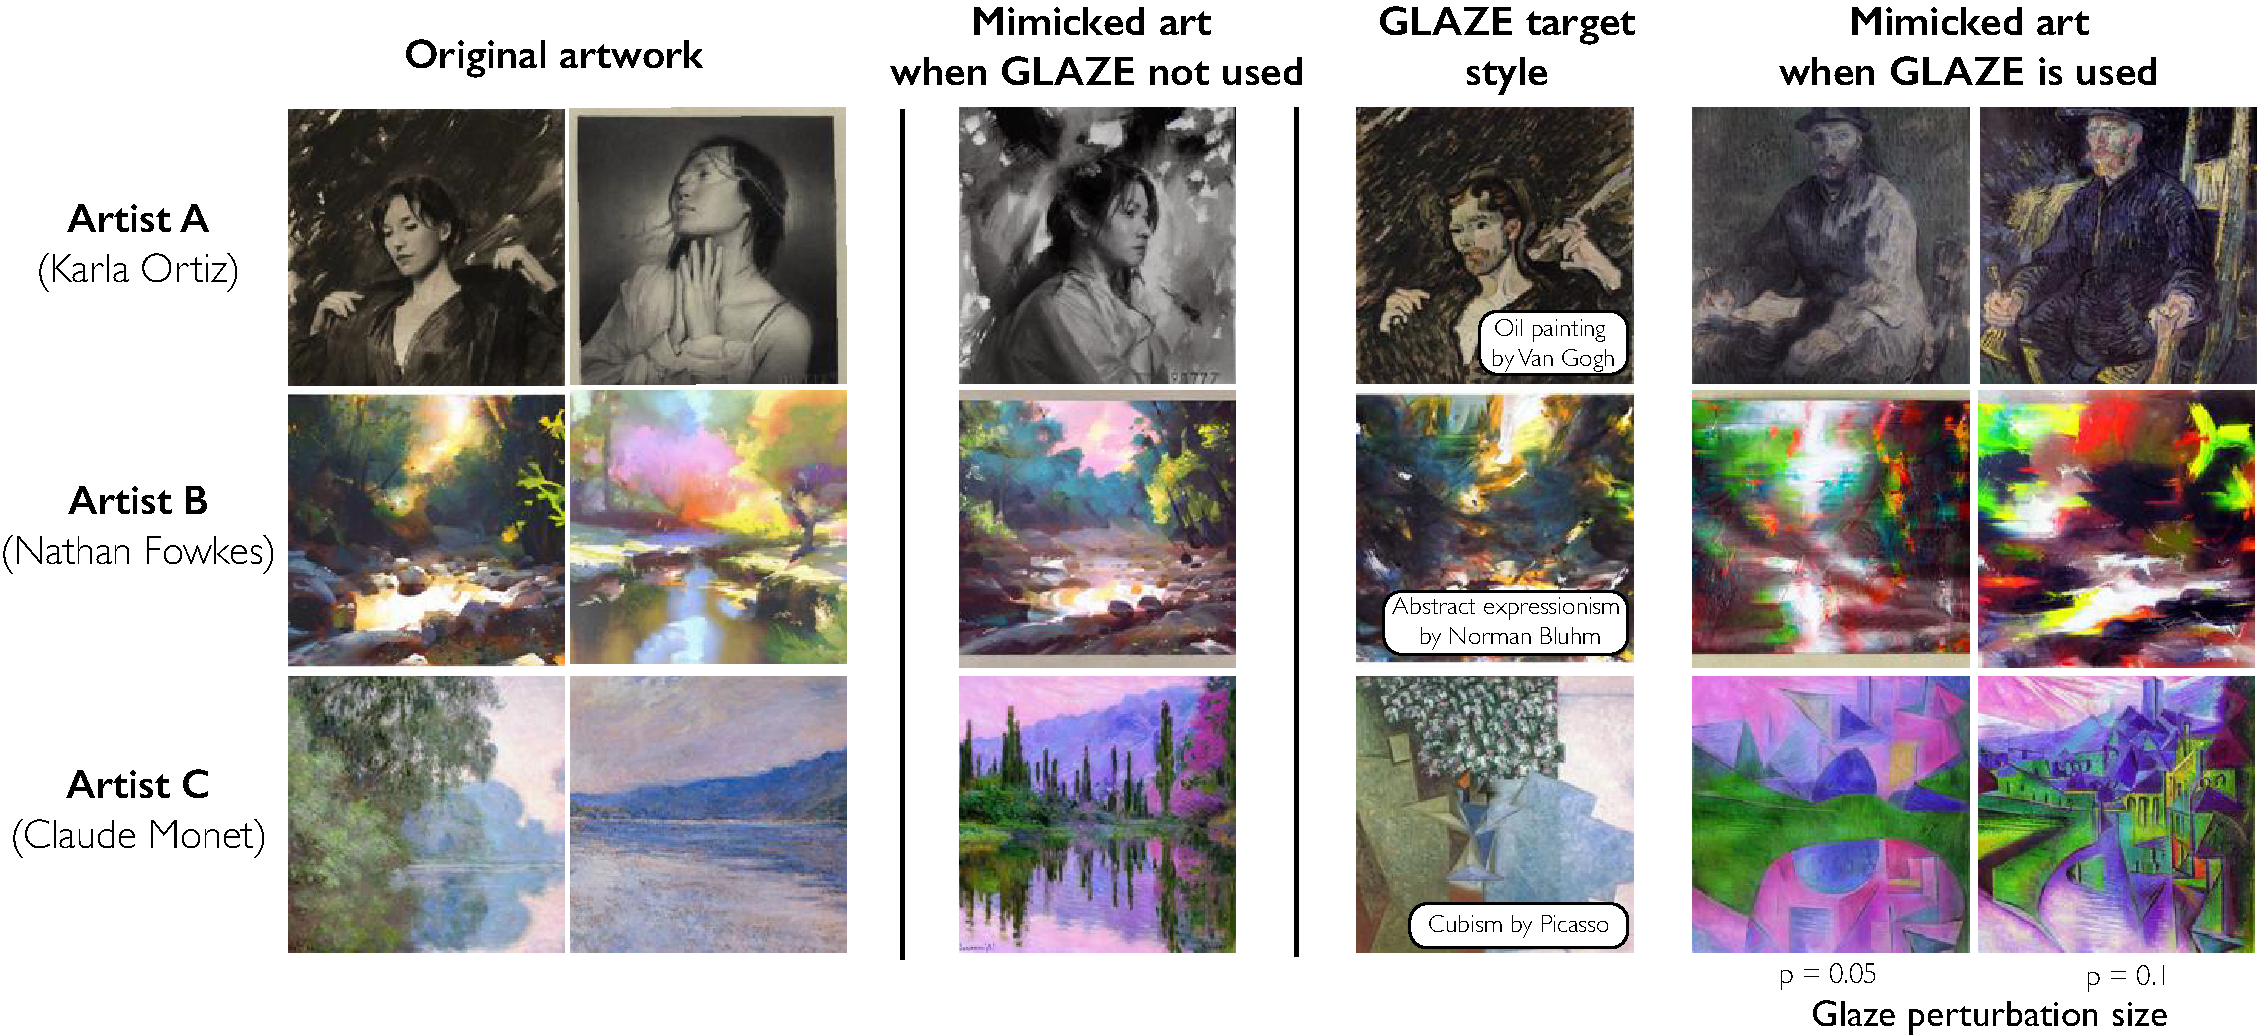
\includegraphics[width=0.9\linewidth]{plots/eval/big-result-full-emily.pdf}
  \vspace{-0.1in}
  \caption{Example \system{} protection results for three artists. {\bf
      Columns 1-2}: artist's original artwork; {\bf column 3}: mimicked
    artwork when artist does not use protection; {\bf column 4}:
    style-transferred artwork (original artwork in column 1 is the source)
    used for cloak optimization and the name of target style; {\bf column
      5-6}: mimicked artwork when artist uses cloaking protection with
    perturbation budget $p=0.05$ or $p=0.1$ respectively. All mimicry
    examples here use SD-based models.
  } %The images can be zoomed for a closer look when viewing the paper digitally. )}
  \label{fig:core-res}
\end{figure*}

\begin{table}[t]
  \centering
  \resizebox{0.5\textwidth}{!}{
  \centering
\begin{tabular}{cccccc}
\toprule
\multirow{2}{*}{\textbf{\begin{tabular}[c]{@{}c@{}} \\ Generic \\ model\end{tabular}}} & \multirow{2}{*}{\textbf{\begin{tabular}[c]{@{}c@{}}\\ Artist \\ dataset\end{tabular}}} & \multicolumn{2}{c}{\textbf{w/o \system{}}} & \multicolumn{2}{c}{\textbf{w/ \system{} (p=0.05)}} \\ \cmidrule{3-6} 
 &  & \begin{tabular}[c]{@{}c@{}}Artist-rated \\ PSR\end{tabular} & \begin{tabular}[c]{@{}c@{}}CLIP-based \\ genre shift\end{tabular} & \begin{tabular}[c]{@{}c@{}}Artist-rated \\ PSR\end{tabular} & \begin{tabular}[c]{@{}c@{}}CLIP-based \\ genre shift\end{tabular} \\ \midrule
\multirow{2}{*}{SD} & Current & $4.6 \pm 0.3\%$ & $2.4 \pm 0.2\%$ & $94.3 \pm 0.8\%$ & $96.4 + 0.5\%$ \\
 & Historical & $4.2 \pm 0.2\%$ & $1.3 \pm 0.2\%$ & $93.3 + 0.6\%$ & $96.0 + 0.3\%$ \\ \midrule
\multirow{2}{*}{\dalleM~} & Current & $31.9 \pm 3.5\%$ & $6.4 \pm 0.8\%$ & $97.4 \pm 0.2\%$ & $97.4 + 0.3\%$ \\
 & Historical & $29.8 \pm 2.4\%$ & $5.8 \pm 0.6\%$ & $96.8 \pm 0.3\%$ & $97.1 + 0.2\%$ \\ \bottomrule
\end{tabular}
  }
  \vspace{-0.1in}
  \caption{\system{} has a high protection success rate, as measured by
    artists and CLIP, against style mimicry attacks. We compare protection
    success when artists do not use \system{} vs. when they do (with
    perturbation budget 0.05). }
  \label{tab:psr-core-table}
  \vspace{-0.3cm}
\end{table}

\begin{figure*}[t]
  \centering
  \begin{minipage}{0.32\textwidth}
  \centering
  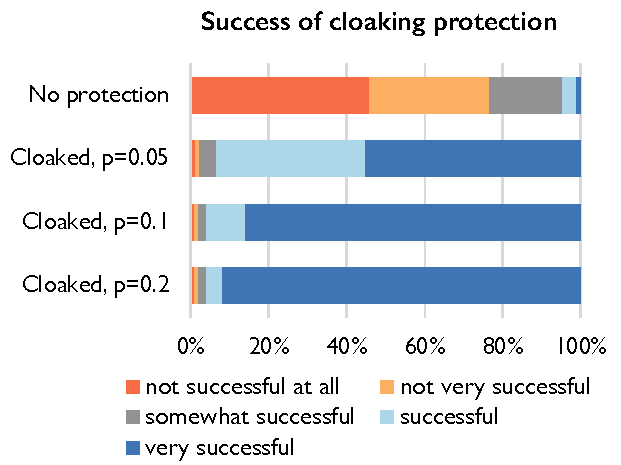
\includegraphics[width=1\columnwidth]{plots/eval/user-cloak-budget.pdf}
  \vspace{-0.23in}
  \caption{\system{}'s cloaking protection success increases as cloak perturbation budget increases. The top row of the figure shows baseline performance with the mimic trains on uncloaked images (p=0). }
  \label{fig:budget-increase}
  \end{minipage}
  \hfill
    \centering
    \begin{minipage}{0.32\textwidth}
  \vspace{0.23in}
  \centering
    \resizebox{1\textwidth}{!}{
    \begin{tabular}{lcc}
    \toprule
    \multicolumn{1}{c}{\textbf{\begin{tabular}[c]{@{}c@{}}Perturbation\\ budget\end{tabular}}} & \textbf{\begin{tabular}[c]{@{}c@{}}Artist-rated \\ PSR\end{tabular}} & \textbf{\begin{tabular}[c]{@{}c@{}}CLIP-based \\ genre shift\end{tabular}} \\ \midrule
    0 (no cloak) & $4.6 \pm 1.4\%$ & $2.4 \pm 0.8\%$ \\
    0.05 & $93.3 \pm 0.6\%$ & $96.0 \pm 0.3\%$ \\
    0.1 & $95.9 \pm 0.4\%$& $98.2 \pm 0.1\%$ \\
    0.2 & $96.1 \pm 0.3\%$ & $98.5 \pm 0.1\%$ \\ \bottomrule
    \end{tabular}
    }
    \vspace{0.13in}
    \captionof{table}{Performance of our system (artist-rated protection success rate and CLIP-based genre shift rate) increases as the perturbation budget increases. (SD model, averaged over all victim artists). }
    \label{tab:budget-increase-sd}
  \end{minipage}
  \hfill
\centering
  \begin{minipage}{0.32\textwidth}
  \centering
  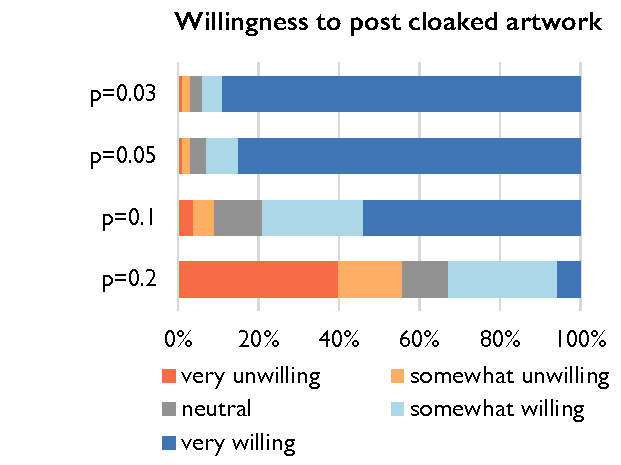
\includegraphics[width=1\columnwidth]{plots/eval/user-accept.pdf}
  \vspace{-0.23in}
  \caption{Artists' willingness to post cloaked artwork in place of the original decreases as perturbation budget of the cloaks increases. }
  \label{fig:artist-accept} 
  \end{minipage}
    \hfill
\end{figure*}

\begin{figure}[t]
  \centering
  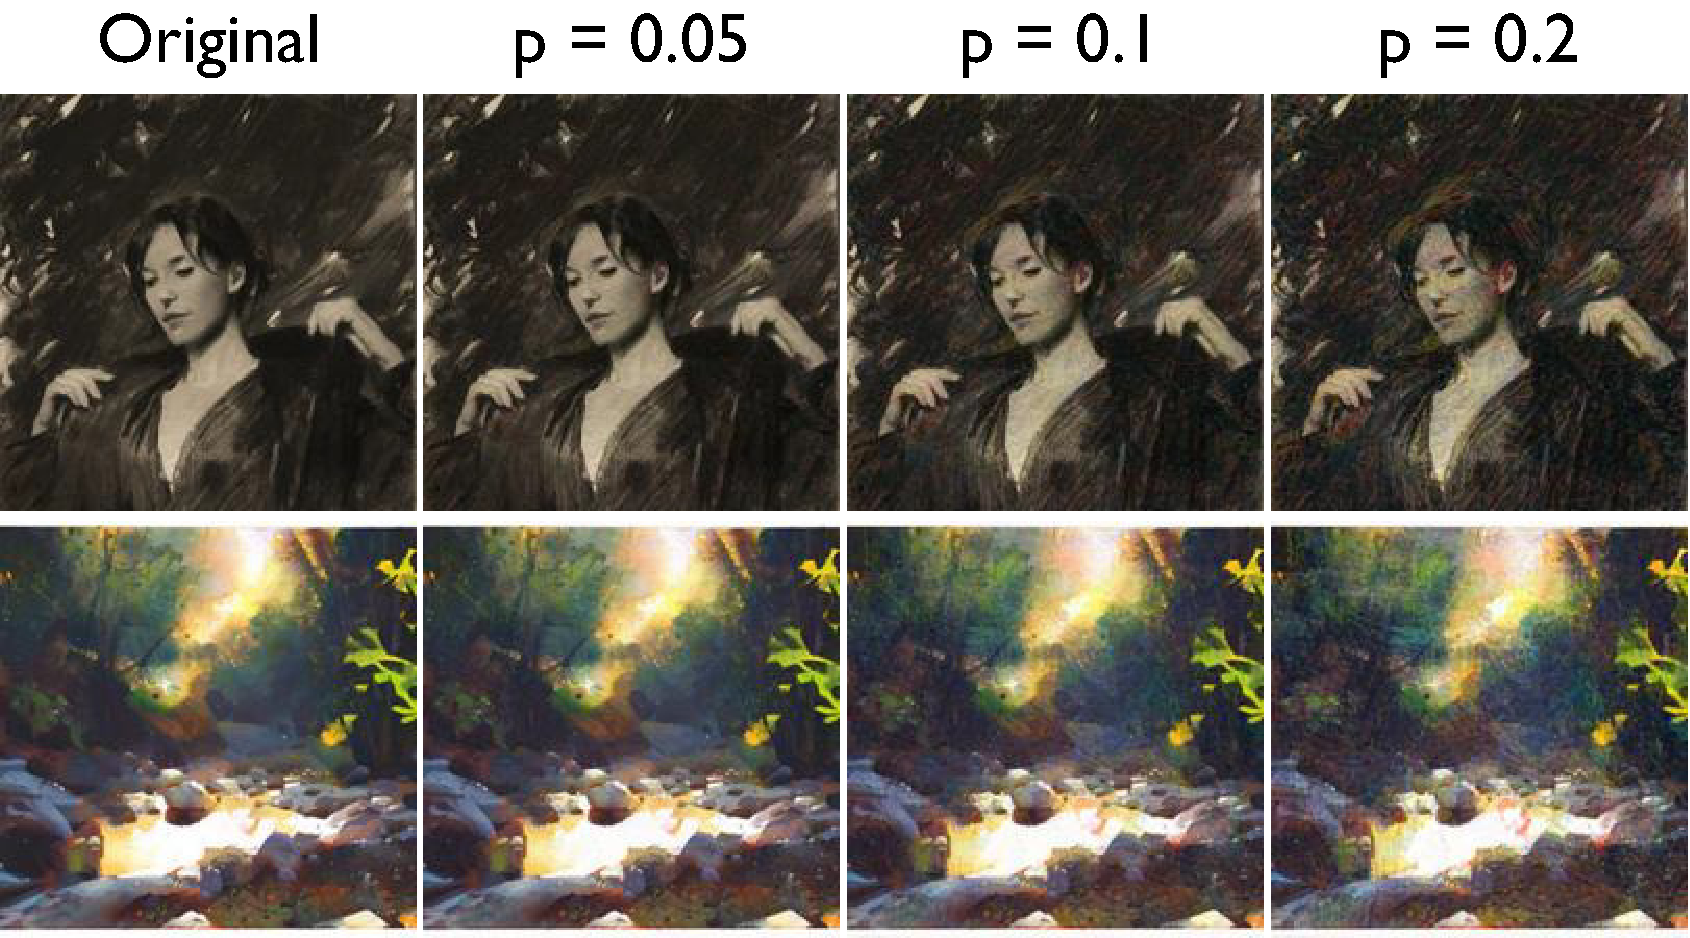
\includegraphics[width=0.90\columnwidth]{plots/eval/cloak-perturbation.pdf}
  \vspace{-0.08in}
  \caption{Original artwork and cloaked artwork computed using three different cloak perturbation budgets. }
  \label{fig:before-after}
\end{figure}

\secspace
\subsection{\system{}'s Protection Performance}
\label{sec:cloaking-results}

\para{Style mimicry success when \system{} is not used. } Mimicry attacks are
very successful when the mimic has access to a victim's original (unmodified)
artwork. Examples of mimicked artwork can be found in
Figure~\ref{fig:core-res}. The leftmost two columns of Figure~\ref{fig:core-res} show a
victim artist's original artwork, while the third column depicts mimicked
artwork generated by a style-specific model trained on victim's original
artwork when \system{} is not used. In our user study, over $>95\%$ of
respondents rated the attack as successful. Table~\ref{tab:psr-core-table},
row 1, gives the artist-rated and CLIP-based genre shift for mimicry attacks on
unprotected art. 

SD models produce stronger mimicry attacks than \dalleM{} models, according
to our user study (see Table~\ref{tab:psr-core-table}). This is unsurprising,
as \dalleM{} models generally produce lower-quality generated
images. CLIP-based genre shift does not reflect this phenomenon, as this metric does
not assess image quality.  

\para{\system{}'s success at preventing style mimicry. } \system{} makes
mimicry attacks markedly less successful, as shown in
Figure~\ref{fig:core-res}. Columns 5 and 6 (from left) show mimicked artwork
when the style-specific models are trained on artwork protected by
\system{}. For reference, column 4 shows an example style-transferred artwork
$\Omega(x, T)$ used to compute \system{} cloaks for the protected art
pieces. Overall, \system{} achieves $> 93.3\%$ artist-rated PSR and
$> 96.0\%$ CLIP-based genre shift (see Table~\ref{tab:psr-core-table}). \system{}'s
protection performance is slightly higher for current artists than for
historical artists. This is likely because the historical artists' images are
present in the training datasets of our generic models (SD, \dalleM),
highlighting the additional challenge of protecting well-known artists whose
style was already learned by the generic models.

\para{How large of perturbations will artists tolerate?} Increasing the
\system{} perturbation budget enhances protection performance. We observe
that both artist-rated and CLIP-based genre shift increase with perturbation budget
(see Figure~\ref{fig:budget-increase}, Table~\ref{tab:budget-increase-sd},
and Figure~\ref{fig:budget2results}). Given this tradeoff between protection
success and \system{} protection visibility on original artwork, we evaluate
how perturbation size impacts artists' willingness to use \system{}. 

We find that artists are willing to add fairly large \system{} perturbations
to their artwork in exchange for protection against mimicry. To measure this,
we show $3$ randomly chosen pairs of original/cloaked artwork to each of the
1,156 artists in our first study. For each art pair, we ask the artist
whether they would be willing to post the cloaked artwork (instead of the
original, unmodified version) on their personal website. More than $92\%$ of
artists select ``willing'' or ``very willing'' when $p=0.05$. This number
only slightly increases to $94.3\%$  when $p=0.03$.
Figure~\ref{fig:artist-accept} details artists' preferences as perturbation
budget increases. (see Figure~\ref{fig:before-after} for examples of cloaked
artwork with increasing $p$). Based on these results, we use perturbation
budget $p = 0.05$ for all our experiments, since most artists are willing to
tolerate this perturbation size.  

Surprisingly, over $32.8\%$ artists are willing to use cloaks with $p=0.2$,
which is clearly visible to human eye (see Figure~\ref{fig:before-after}). While we
are surprised by this high perturbation tolerance, in our follow-up free
response artists noted that they would be willing to tolerate large
perturbations because of the devastating consequence if their styles are
stolen. One participant stated that ``I am willing to sacrifice a bit image
quality for protection.'' Many artists ($>80\%$) also noted that they have
already used traditional, more visually disruptive techniques to protect
their artwork online when posting online, \ie adding watermark or reducing
image resolution. One participant stated that ``I already use low to medium
resolution images only for online posting, thus this would not impact my
quality control too much.'' 

\begin{figure*}[t]
  \centering
  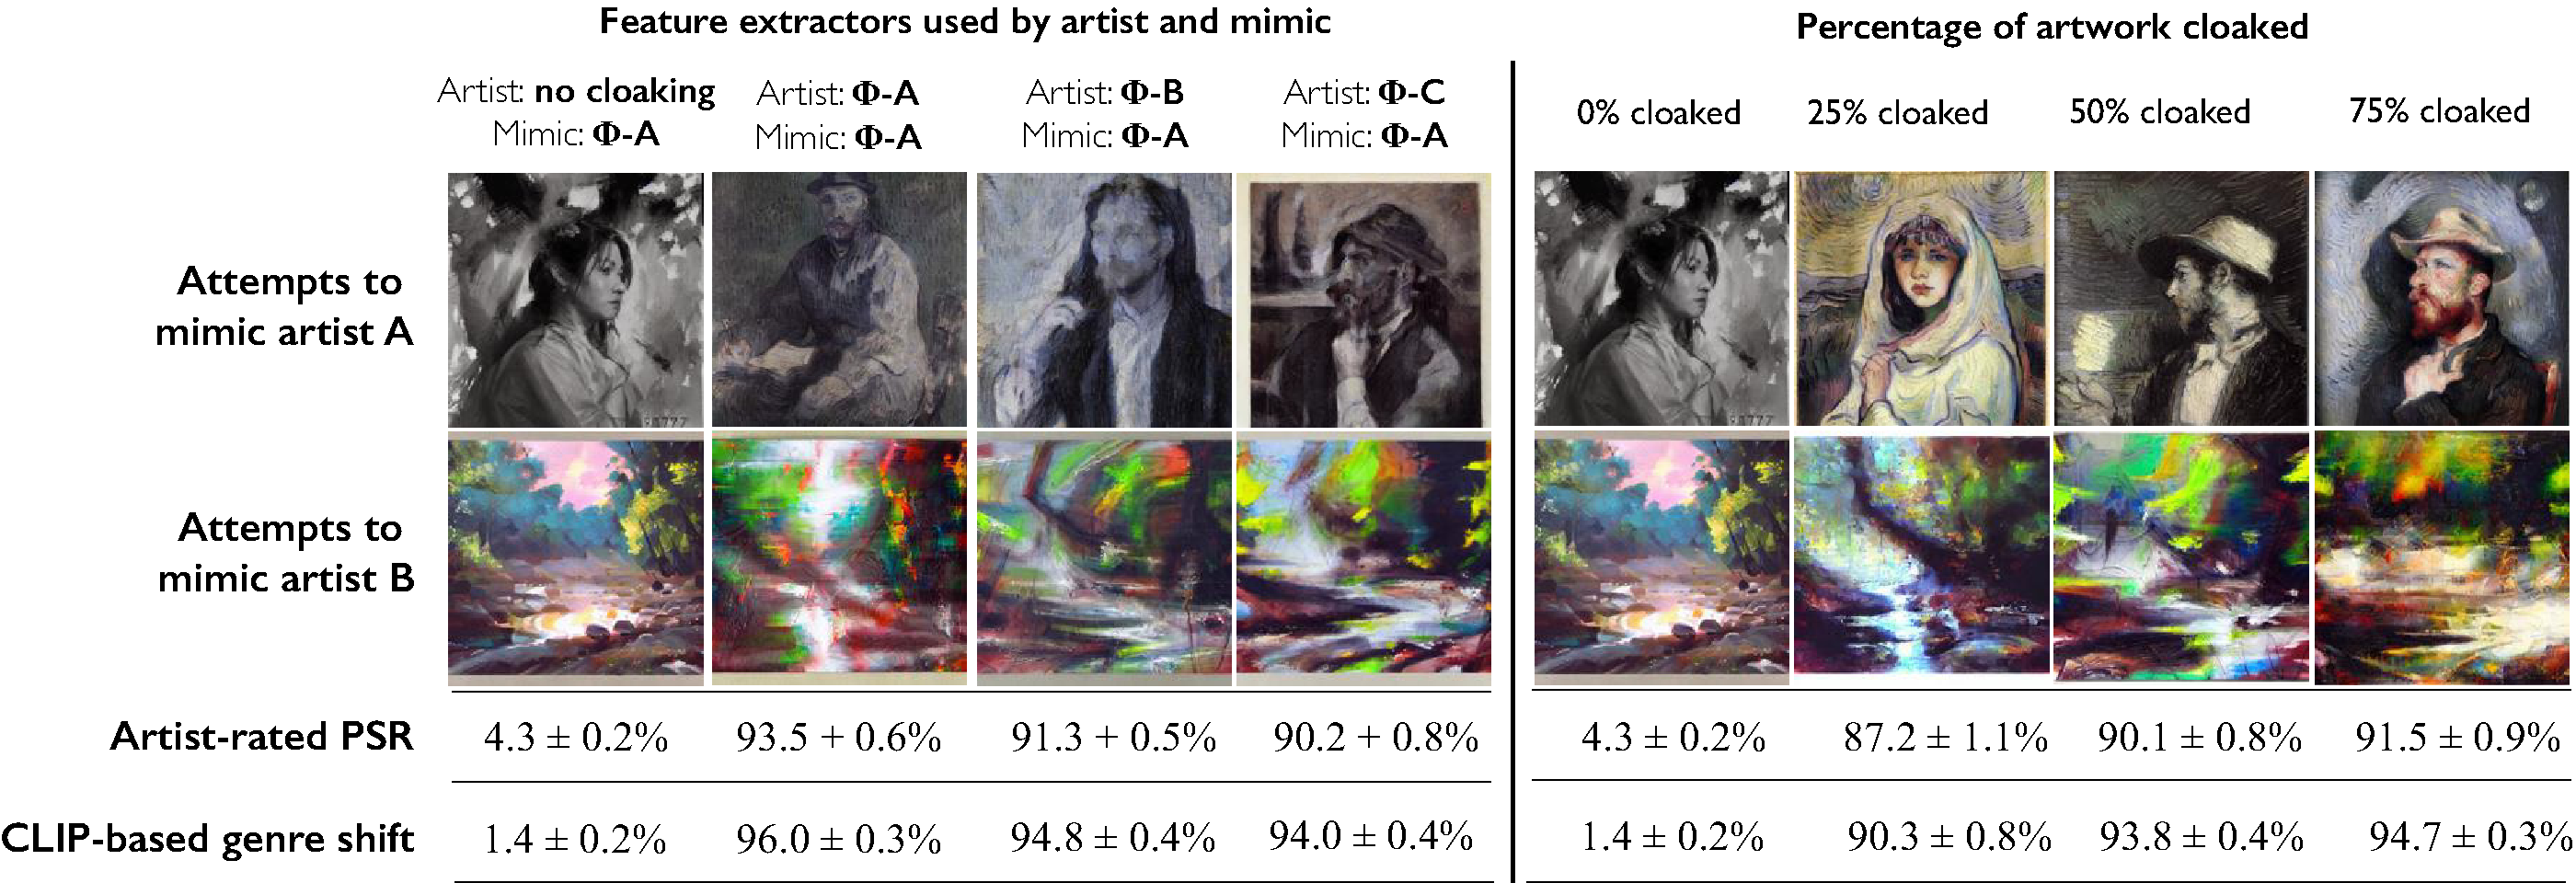
\includegraphics[width=0.95\linewidth]{plots/eval/eval-robust.pdf}
  \caption{\system{} remains successful under two challenging
    scenarios. Left: when artist and mimic use different feature
    extractors. Right: when artists can only cloak a portion of their artwork
    in mimic's dataset. Bottom of the figure shows artist-rated PSR and
    CLIP-based genre shift for the corresponding setting. } 
  \label{fig:core-robust}
\end{figure*}

\secspace
\subsection{\system{}'s Protection Robustness}
\label{sec:robust-eval}

\secspace

Next, we test \system{}'s efficacy in more challenging scenarios. First, we
measure performance when the mimic uses a different feature extractor for
mimicry than the one used by the artist to generate the cloak. Second, we
measure what happens when the mimic has uncloaked artwork samples from the
victim.  Due to the poor mimicry performance of \dalleM, we focus our
evaluation using SD as the generic model.

\para{Artist/mimic use different feature extractors. } In the real world, it
is possible that the mimic will use a different model (and thus a different image
feature extractor) for style mimicry than the one used by the victim artist
to cloak their artwork. While the feature extractors may still be similar
because of the well-known transferability property between large
models~\cite{demontis2019adversarial,transfer,suciu2018does,transfer2014,shan2022post},
their differences could reduce the efficacy of cloaking. We test this
scenario using three feature extractors\textemdash $\Phi$-A, $\Phi$-B, and
$\Phi$-C. $\Phi$-A and $\Phi$-B have different model architectures
(autoencoder-KL~\cite{rombach2022high} vs. VQ-VAE~\cite{ramesh2021zero}) but
are both trained on the ImageNet dataset~\cite{deng2009imagenet}. $\Phi$-A
and $\Phi$-C have different model architectures (autoencoder-KL vs VQ-VAE)
and training datasets (ImageNet vs. CelebA~\cite{liu2018large}).

In our experiments, the victim artist uses one feature extractor (either
$\Phi$-B or $\Phi$-C) to optimize cloaked artwork, and the mimic trains their
style-specific models with SD models using $\Phi$-A. Despite the difference
in victim/mimic extractors, \system{}'s protection remains highly successful
(left half of Figure~\ref{fig:core-robust})\textemdash the style of mimicked
artwork remains distinct from artist's true style. Artist-rated and
CLIP-based genre shift measurements confirm this observation. Artist-rated PSR is
$> 90.2\%$, while CLIP-based genre shift is $> 94.0\%$. The PSR is slightly higher
when the two feature extractors only differ in architectures ($\Phi$-B to
$\Phi$-A) than when they differ in both architecture and training data
($\Phi$-C to $\Phi$-A).


\para{Mimic has access to uncloaked artwork. } Another challenging scenario
is when the mimic gains access to some \textit{uncloaked} artwork from victim
artists. This is a realistic scenario for many prominent artists with a large
online presence. As expected, \system{}'s protection performance decreases
when the mimic has access to more uncloaked artwork (right side of
Figure~\ref{fig:core-robust}). As the ratio of uncloaked/cloaked art in the
mimic's dataset increases, the mimicked artwork becomes more similar to
artist's original style. Yet, \system{} is still reasonably effective
($87.2\%$ artist-rated PSR) even when artists can only cloak $25\%$ of their
artwork. This validates our hypothesis in \S\ref{sec:cloak-effect} that
cloaking will have a noticeable effect as long as the mimic has some cloaked
training data.

A mimic with access to a large amount of uncloaked artwork is still an issue
for \system{}. Fortunately, in our user study, we found that 1) many artists
constantly create and share new artwork online, which can be cloaked to
offset the percentage of uncloaked artwork, and 2) many artists change their
artistic style over time. In our user study, we asked artists to estimate the
number of unique art pieces they currently have online ($M$) and the
estimated number of art pieces they anticipate uploading each subsequent year
($Y$). Among artists with an existing online presence, over $40\%$ have
$Y / M > 25\%$, meaning that one year from now, $> 20\%$ of their total
online artwork would be cloaked (if they start using \system{}
immediately). More than $81\%$ of artists also stated that their art style
has changed over their career, and half of these said that theft of their
old, outdated styles is less concerning.


\begin{table}[t]
  \centering
  \resizebox{0.49\textwidth}{!}{
  \centering
  \begin{tabular}{ccccc}
    \hline
    \multirow{2}{*}{\textbf{\begin{tabular}[c]{@{}c@{}}Artist \\ dataset\end{tabular}}} & \multicolumn{2}{c}{\textbf{w/o \system}} & \multicolumn{2}{c}{\textbf{w/ \system{} (p=0.05)}} \\ \cline{2-5} 
     & \begin{tabular}[c]{@{}c@{}}Artist-rated \\ PSR\end{tabular} & \begin{tabular}[c]{@{}c@{}}CLIP-based \\ genre shift\end{tabular} & \begin{tabular}[c]{@{}c@{}}Artist-rated \\ PSR\end{tabular} & \begin{tabular}[c]{@{}c@{}}CLIP-based \\ genre shift\end{tabular} \\ \hline

    Current & $6.2 \pm 0.5\%$ & $3.8 \pm 0.3\%$ & $92.5 \pm 0.5\%$ & $94.2 + 0.3\%$ \\
    Historical & $7.2 \pm 0.6\%$ & $3.3 \pm 0.4\%$ & $92.1 + 0.3\%$ & $93.9 + 0.4\%$ \\ 
    \hline
    \end{tabular}
  }
  \vspace{-0.1in}
  \caption{Performance of \system{} against real-world mimicry service
    (scenario.gg). Mimicry service achieves high mimicry success when no
    protection is used. When \system{} is used, the mimicry service has low
    performance. }
  \label{tab:real-world}
\end{table}

\secspace
\subsection{Real-World Performance}

Next, we test \system{} against a real-world style mimicry-as-a-service
system, \texttt{scenario.gg}~\cite{aigame}. Scenario.gg is a web service that
allows users to upload a set of images in a specific style. The
service then trains a model to mimic the style and returns an API endpoint
that allows the user to generate mimicked images in the trained style. The
type of model or mimicry method used by the service is unknown.

\system{} remains effective against \texttt{scenario.gg}. We ask
\texttt{scenario.gg} to mimic the style from a set of cloaked or uncloaked
artwork from $4$ current artists and $19$ historical
artists. Table~\ref{tab:real-world} shows that when no protection is used,
\texttt{scenario.gg} can successfully mimic the victim style (< 7.2\%
protection success). The mimicry success of \texttt{scenario.gg} is lower
than our mimicry technique, likely because \texttt{scenario.gg} trains the
model for fewer iterations due to computational constraints. When we use
\system{} to cloak the artwork and upload the cloaked artwork,
\texttt{scenario.gg} fails to mimic the victim style ($> 92.1\%$ artist-rated
PSR and $> 93.9\%$ CLIP-based genre shift rate) as shown in Table~\ref{tab:real-world}.
